\chapter{Forecasting Limit Order Books with CNN-LSTM Architectures}

As a future methodology to explore, they also mention a CNN-LSTM Architecture given by \cite{cutuli_trading_lob_cnn_lstm}. This work explores a combined CNN-LSTM network to classify future directions of the order book at high frequency, drawing heavy inspiration from the work of Zhang et al. \cite{zhang2019deeplob} and Kolm et al. \cite{kolm2021deepofi}. The primary goal is to predict whether the mid-price increases, decreases, or does not change in the very next observation. 

\section{Problem Setup}

They represent the limit order book using the first ten levels of market depth. Each observation is a 40-variable vector containing the prices and volumes for the top ten bids and asks. 

A sequence of raw limit order book states is a complex non-stationary process. To address this, they transform the raw data into order flow and order flow imbalance. Order flow is a 20-variable vector that computes changes between consecutive states while keeping the bid and ask sides separate. Order flow imbalance is a 10-variable vector calculated by simply subtracting the ask order flow from the bid order flow. 

These formulas transform the sequence into a stationary process. This stationary property allows the LSTM to learn long-term dependencies much more easily. Furthermore, training on order flow gives the CNN layers the flexibility to combine bid and ask flows asymmetrically. Because of this, the forecasting models are expected to perform better on order flow than on order flow imbalance.

\section{The CNN-LSTM Architecture}
\begin{figure}[h
]
    \centering
    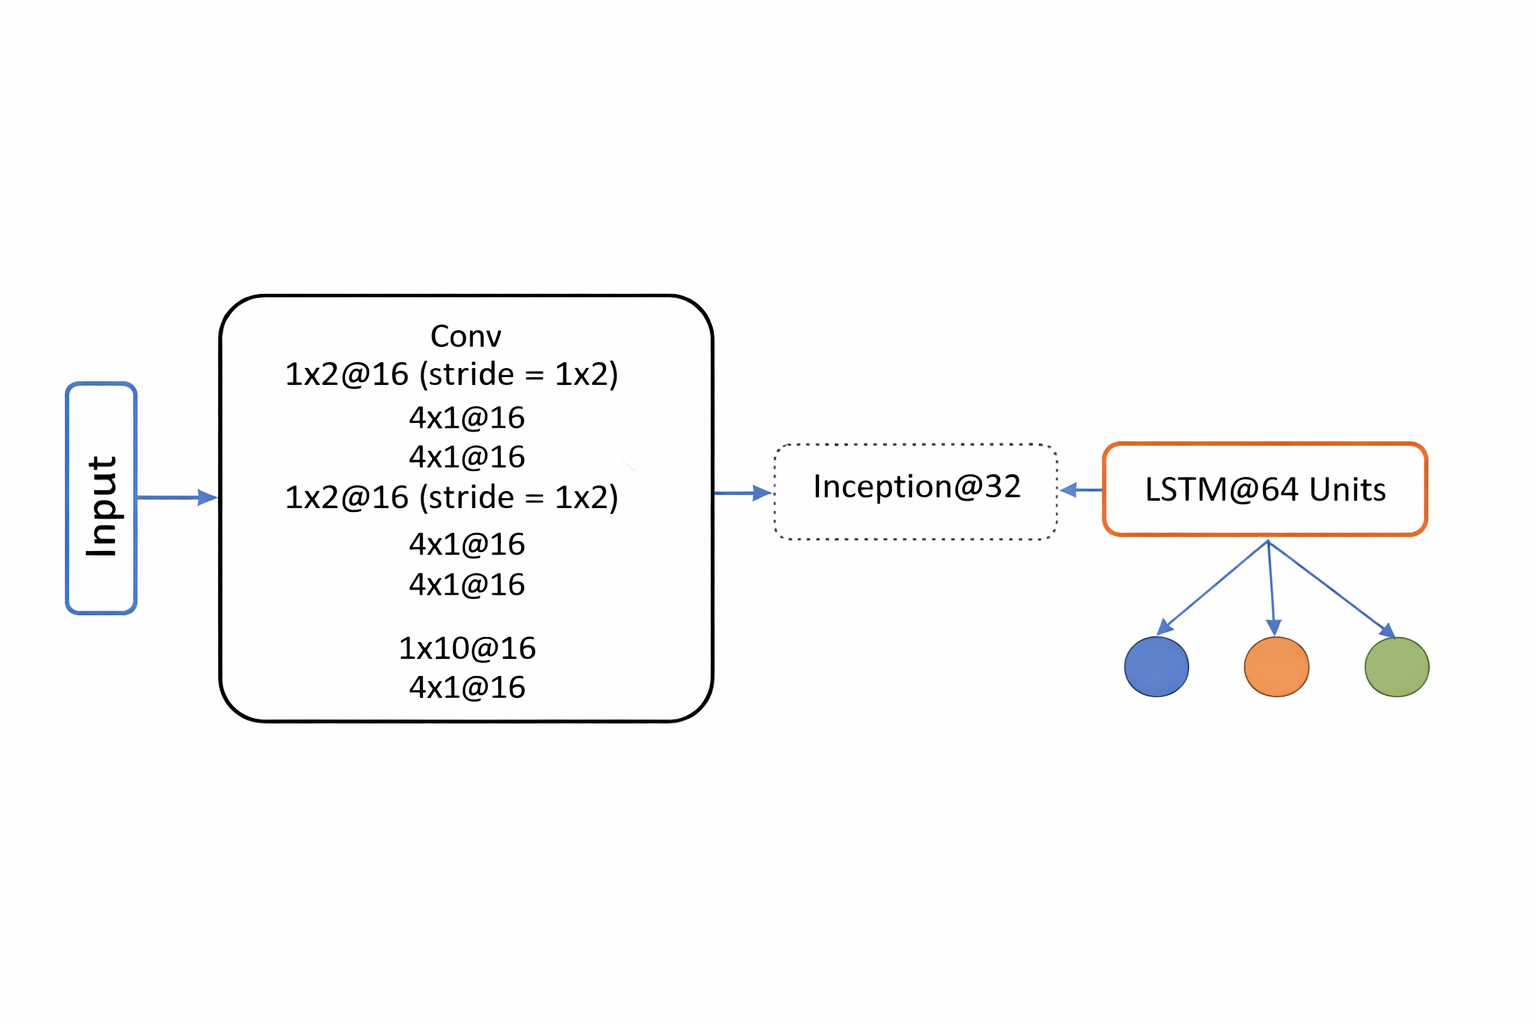
\includegraphics[width=0.82\linewidth]{CNN LSTM Architecture.png}
    \caption{Architecture of the CNN LSTM Model as mentioned by Zhang et al. \cite{zhang2019deeplob}}
    \label{fig:cnnlstmarch}
\end{figure}
Different neural network architectures are highly complementary. When used together, they can learn unique structures in the data and improve the model's ability to execute a desired task.

The CNN layers first reduce the dimensionality of the multivariate input by aggregating the sides and levels of the order book. The output of these convolutions feeds directly into an Inception Module. This module wraps convolutions together to capture market behavior across multiple timescales. It serves as a moving average indicator where the decay weights are learned via backpropagation. 

The outputs from the Inception Module are then concatenated and reshaped into a sequence. This sequence serves as the input to the LSTM layer. The LSTM learns the temporal dependencies from this compressed parameter space, leading to a much more parsimonious model. 

They formulate this forecasting problem as one of classification. They add an output layer with a softmax activation function to output the estimated probability for each price movement. The authors also apply Monte-Carlo (MC) dropout as a stochastic regularizer. This reduces overfitting and allows the model to take epistemic uncertainty into account.

\section{Methodology and Training}

The authors adopt a Box-Jenkins approach for modeling the time series. They initially fit Vector Autoregressive (VAR) models to the data. They select the optimal lag order by minimizing the Akaike Information Criterion (AIC). This helps infer how long our LSTM lookback window should be.

They tune the dropout hyperparameters using a  brute-force search looking for the best loss value from the dropout set of [0.1, 0.2, 0.3, 0.4, 0.5] for the Order Flow (OF) and Order Flow Imbalance (OFI) cases. During the training procedure, they apply early stopping to avoid overfitting. Training terminates automatically if the validation loss fails to improve for five consecutive epochs.

\section{Trading Strategy Evaluation}

To test the models, they perform 100 forward passes using MC dropout on the out-of-sample data, then average the predictions across these passes to approximate the true conditional probability of an outcome. They then compare two intra-second trading strategies. For each timestamp they trade at, they size our position at 30\% of the volume available at the entry level.

The Softmax Strategy relies on a chosen probability threshold. The strategy goes long if the probability of an upward move exceeds the threshold, and it goes short if the probability of a downward move exceeds the threshold. 

The Bayesian Strategy leverages predictive entropy to summarize classification uncertainty. Predictive entropy is minimized when the model is absolutely certain about one class. The entropy is maximized when probabilities are uniform across the classes. This strategy upsizes positions when the model is certain, downsizes positions when the model is uncertain, and exits the position entirely if the model becomes highly uncertain.

\section{Results and Diagnostics}

% \begin{figure}[h
% ]
%     \centering
%     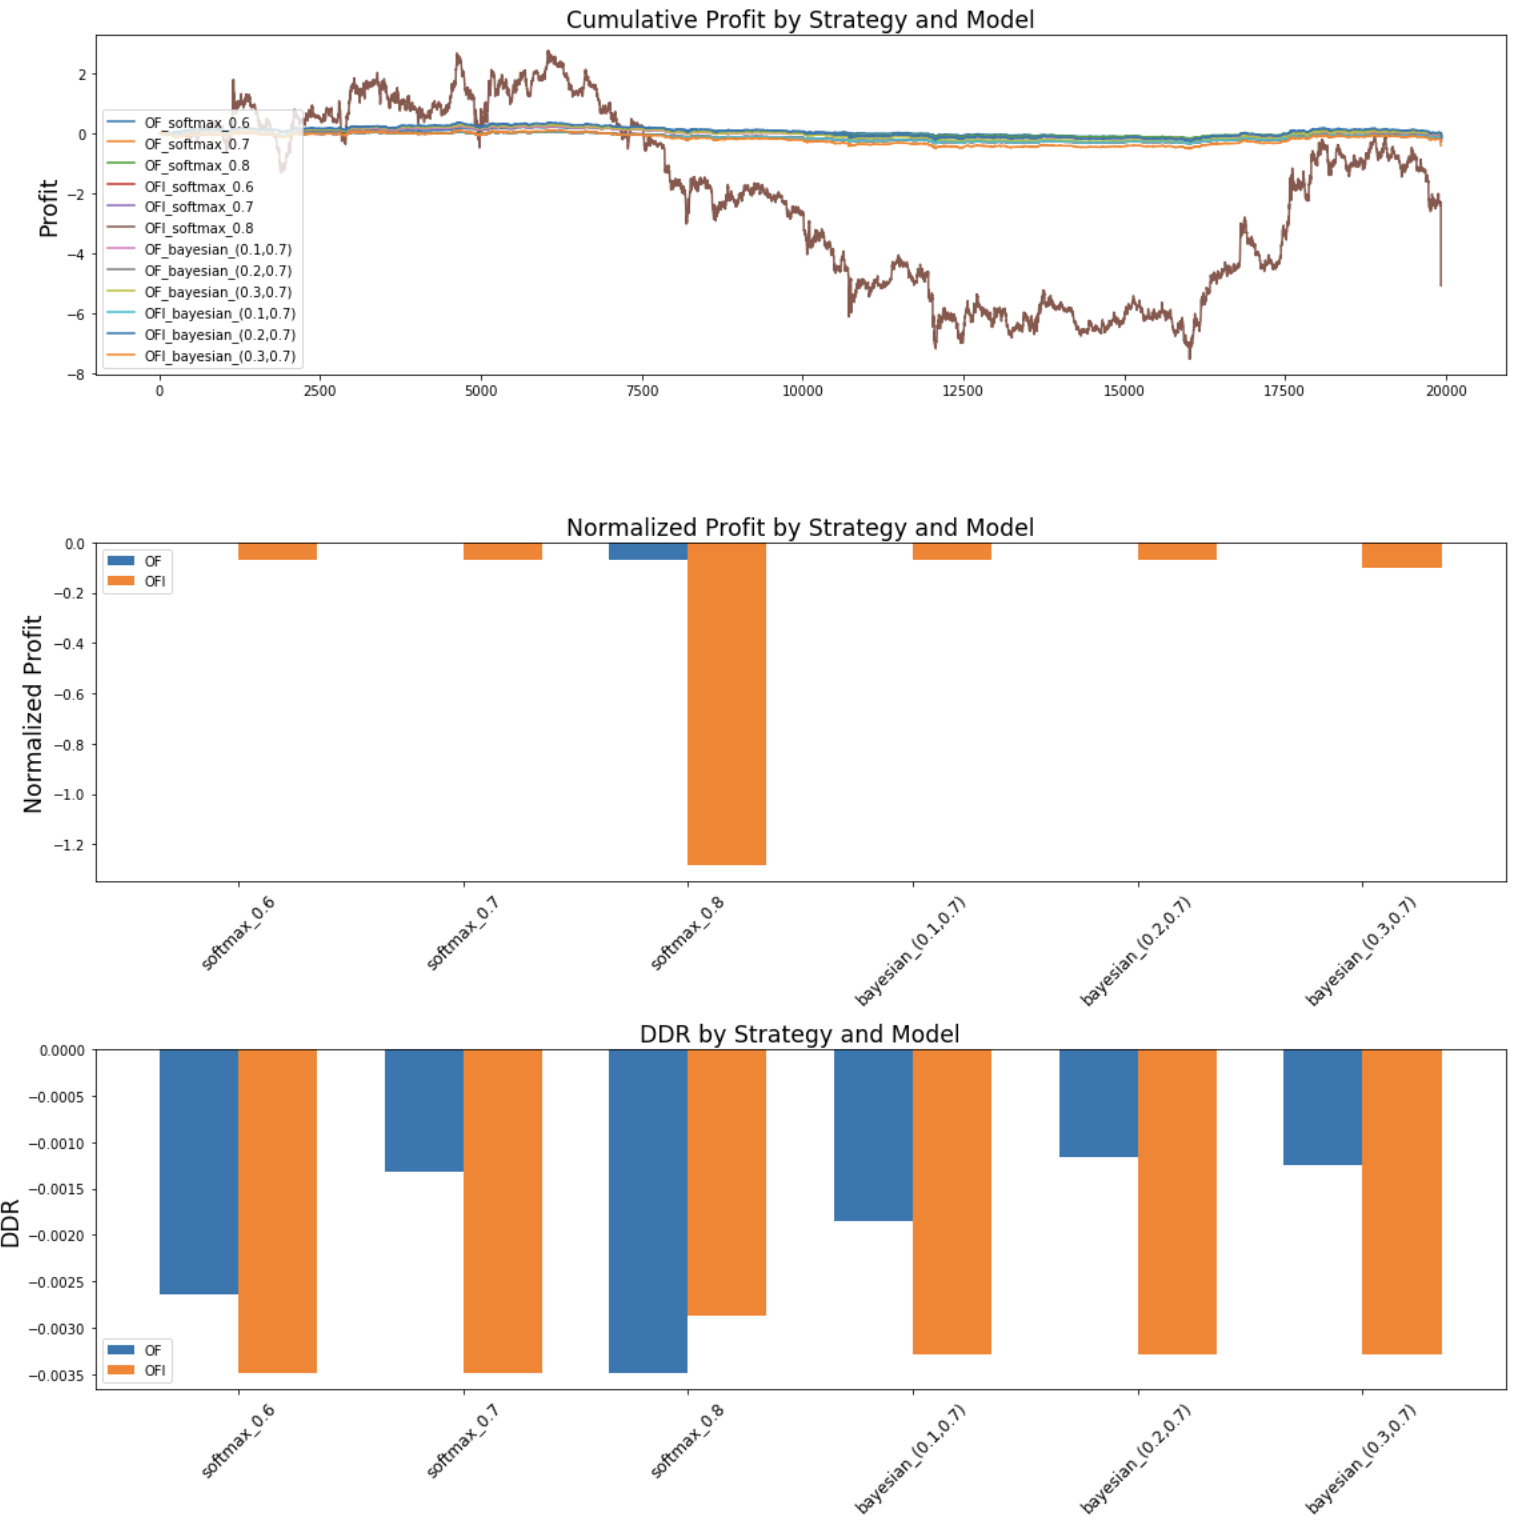
\includegraphics[width=0.82\linewidth]{Cutuli Results.png}
%     \caption{Results mentioned in the article by Cutuli\cite{cutuli_trading_lob_cnn_lstm}}
%     \label{fig:resultscutuli}
% \end{figure}
They compare the strategies using standardized profits and the Downward Deviation Ratio (DDR). DDR serves as our risk measure because it appropriately penalizes negative returns while rewarding positive returns.

Both models performed poorly in generating raw profits. The Bitcoin mid-price dropped by 1\% over the duration of the trading period. Because the models were poor at predicting downward moves, they were doomed to behave poorly in this downward trending regime. Proper downsampling during training would have helped the model predict these downward moves.

Despite the trading losses, the Bayesian strategy remained much steadier than the Softmax strategy. This indicates that incorporating model uncertainty is highly beneficial. Normalized profits also clearly illustrated that training on order flow significantly outperforms training on order flow imbalance.

Finally, they performed model diagnostics using the Ljung-Box test. They tested the sample autocorrelations of the model residuals, computed via cross-entropy. The test provided statistical evidence to reject the null hypothesis of white noise. This indicates that the models underfit the training data. Financial data is incredibly complex, and it is highly difficult for any interpretable model to perfectly fit the input data.